\documentclass[a4paper,12pt]{report}
\usepackage[utf8]{inputenc}
\usepackage[francais]{babel}
\usepackage{fancyhdr}
\usepackage{graphicx}
\usepackage{tikz}
\usetikzlibrary{calc}
\usepackage{listings}
\usepackage{xcolor}
\definecolor{grey}{rgb}{0.9,0.9,0.9}
\usepackage{titlesec}
\usepackage{verbatim}
\usepackage{listings}
\usepackage{textcomp}
\usepackage{hyperref}
\usepackage{amssymb}
\usepackage{amsmath}
\usepackage{longtable}
\usepackage{colortbl}
\usepackage{float}
\usepackage{caption}
\usepackage{subfig}
\usepackage{color}


\lstset{ %
  language=R,                     % the language of the code
  basicstyle=\footnotesize,       % the size of the fonts that are used for the code
  numbers=left,                   % where to put the line-numbers
  numberstyle=\tiny\color{gray},  % the style that is used for the line-numbers
  stepnumber=1,                   % the step between two line-numbers. If it's 1, each line
                                  % will be numbered
  numbersep=5pt,                  % how far the line-numbers are from the code
  backgroundcolor=\color{white},  % choose the background color. You must add \usepackage{color}
  showspaces=false,               % show spaces adding particular underscores
  showstringspaces=false,         % underline spaces within strings
  showtabs=false,                 % show tabs within strings adding particular underscores
  frame=single,                   % adds a frame around the code
  rulecolor=\color{black},        % if not set, the frame-color may be changed on line-breaks within not-black text (e.g. commens (green here))
  tabsize=2,                      % sets default tabsize to 2 spaces
  captionpos=b,                   % sets the caption-position to bottom
  breaklines=true,                % sets automatic line breaking
  breakatwhitespace=false,        % sets if automatic breaks should only happen at whitespace
  title=\lstname,                 % show the filename of files included with \lstinputlisting;
                                  % also try caption instead of title
  keywordstyle=\color{blue},      % keyword style
  commentstyle=\color{green},   % comment style
  stringstyle=\color{magenta},      % string literal style
  escapeinside={\%*}{*)},         % if you want to add a comment within your code
  morekeywords={*,...}            % if you want to add more keywords to the set
} 


\frenchbsetup{StandardLists=true}
\newcommand{\marge}{18mm}
\usepackage[left=\marge,right=\marge,top=\marge,bottom=\marge]{geometry}
\pagestyle{fancy}
\setlength{\headheight}{14pt}
\chead{
  \textbf{Binôme :} Douaille Erwan \& François Rémy
  \hspace{2em}
  \textbf{Groupe :} M1 Info RDF}
\renewcommand{\headrulewidth}{1pt}
\linespread{1}
\setlength{\columnseprule}{0.2pt}





\begin{document}


\makeatletter
\begin{titlepage}
\centering
\vspace{-10em}
{\LARGE \textbf{\textsc{Rapport de Projet RVI}}}\\
\vspace{3em}

\includegraphics[scale=0.6]{image/thalassa.png}\\
\vspace{3em}
{\LARGE \textsc{Projet Thalassa: simulation de plongée sous-marine}}\\

\vspace{8em}
Par\\
\vspace{1em}
{\LARGE \@author}\\

\vspace{2em}



\begin{tikzpicture}[remember picture,overlay]

\node [below left,xshift=-1cm, yshift=4cm] at (current page.south east){
\includegraphics[scale=0.6]{image/ustl1.png}};

\end{tikzpicture}
\end{titlepage}
\makeatother

\sloppy

\setcounter{page}{1} 
\newpage

%%%%%%%%%%%%%%%%%%%%%%%%%%%%%%%%%%%% INTRODUCTION
%%%%%%%%%%%%%%%%%%%%%%%%%%%%%%%%%%%%%%%%%%%%%%%%%
%%%%%%%%%%%%%%%%%%%%%%%%%%%%%%%%%%%%%%%%%%%%%%%%%
\section*{Introduction}

Le but de ce TP est d'utiliser les fonctions linéaire et quadratique afin de classifier des points en utilisant des données d'apprentissage. Nous allons observer et comprendre comment utiliser ces techniques pour faire de l'analyse discriminante.
	
\section*{Question 1}

\begin{figure}[!ht]
	\center
	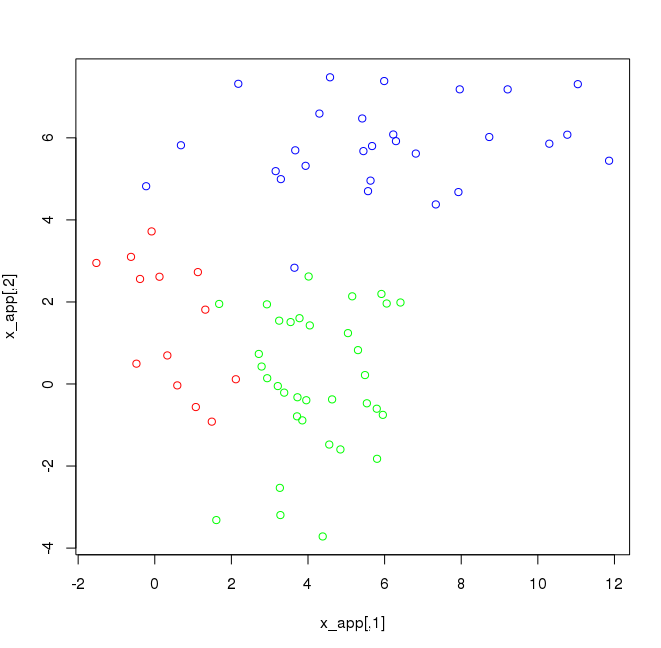
\includegraphics[scale=0.3]{image/q1_1_app.png}
	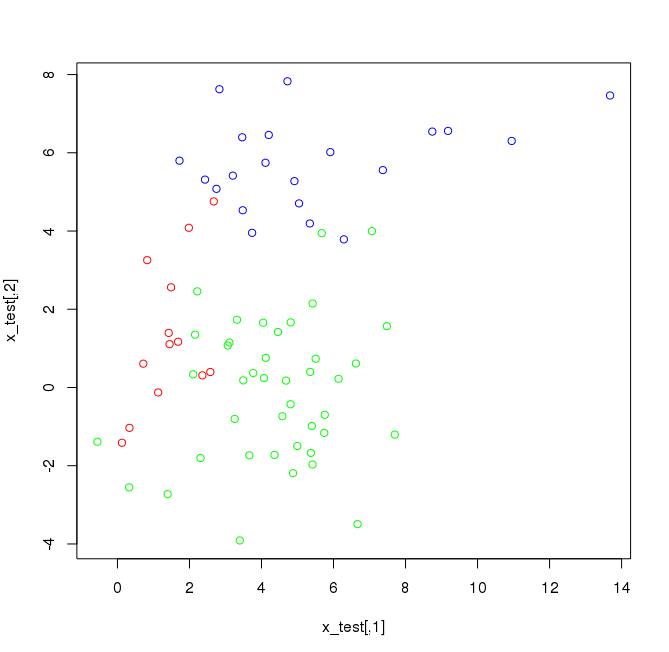
\includegraphics[scale=0.3]{image/q1_1_test.png}
\end{figure}

À gauche les observations de l'application et à droite l'observation de test.
	
\section*{Question 2}

\begin{lstlisting}
print(mean(x_app[classe_app==1,1]))
print(mean(x_app[classe_app==1,2]))
print(mean(x_app[classe_app==2,1]))
print(mean(x_app[classe_app==2,2]))
print(mean(x_app[classe_app==3,1]))
print(mean(x_app[classe_app==3,2]))
\end{lstlisting}

\[M
   \left (
   \begin{array}{cc}
      0.3901397 & 1.483721 \\
      5.979027 & 5.815149 \\
      4.192731 & 0.05827418 \\
   \end{array}
   \right )
\]

\[m
   \left (
   \begin{array}{cc}
      1 & 2 \\
      6 & 6 \\
      4 & 0 \\
   \end{array}
   \right )
\]

Les valeurs ne sont pas les mêmes mais sont sensiblement proches.
\newpage 

\begin{lstlisting}
print(sqrt(cov(as.vector(x_app[classe_app==1,1]),as.vector(x_app[classe_app==1,1]))))
print(sqrt(cov(as.vector(x_app[classe_app==1,2]),as.vector(x_app[classe_app==1,2]))))
print(sqrt(cov(as.vector(x_app[classe_app==2,1]),as.vector(x_app[classe_app==2,1]))))
print(sqrt(cov(as.vector(x_app[classe_app==2,2]),as.vector(x_app[classe_app==2,2]))))
print(sqrt(cov(as.vector(x_app[classe_app==3,1]),as.vector(x_app[classe_app==3,1]))))
print(sqrt(cov(as.vector(x_app[classe_app==3,2]),as.vector(x_app[classe_app==3,2]))))
\end{lstlisting}

\[Sigma
   \left (
   \begin{array}{cc}
      1.017921 & 1.569878 \\
      3.025857 & 1.078742 \\
      1.262385 & 1.708196 \\
   \end{array}
   \right )
\]

\[s
   \left (
   \begin{array}{cc}
      1 & 2 \\
      3 & 1 \\
      1.5 & 2 \\
   \end{array}
   \right )
\]

Comme précédemment les valeurs ne sont pas les mêmes mais les écarts sont plutôts proche.

Les attributs ne sont pas indépendants, on l'a constaté avec les calculs ci-dessous.

\section*{Question 3}
Nous obtenons un taux de bonne classification de 0.84
	
\begin{figure}[!ht]
	\center
	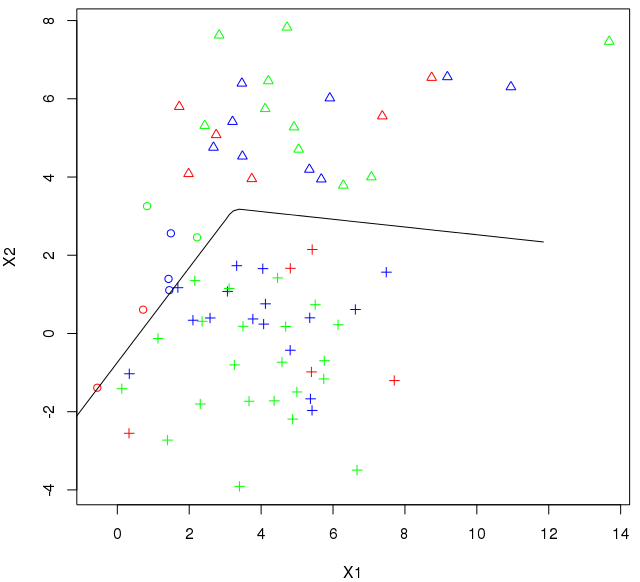
\includegraphics[scale=0.5]{image/q3.png}
\end{figure}

La classification nous à permis d'obtenir les résultats avec des formes. Ces formes ont ensuite été séparé grâce à la fonction de décision pour la classe 1 et 2. Si on avait utilisé une fonction de décision pour la classe 1 et 3 par exemple on aurait clairement eu une délimitation entre les différentes formes présente sur le canvas.

\section*{Question 4}
Nous obtenons un taux de bonne classification de 0.9066667
	
\begin{figure}[!ht]
	\center
	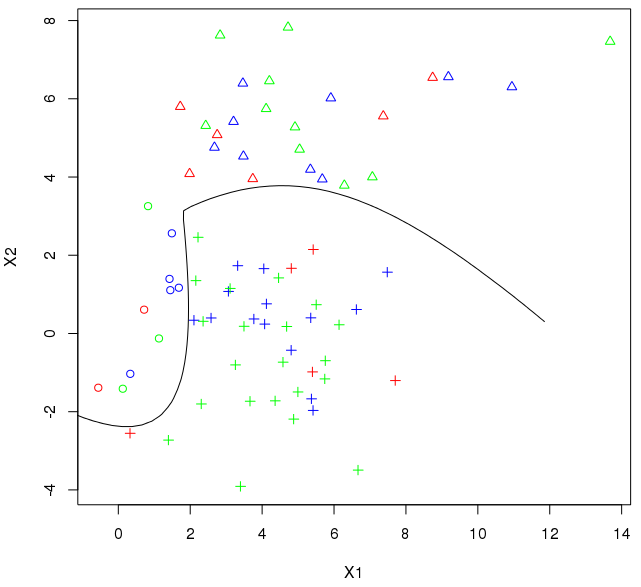
\includegraphics[scale=0.5]{image/q4.png}
\end{figure}

En utilisant une fonction quadratique plutôt qu'une linéaire, nous obtenons un taux de bonne classification plus élevé. Nous constatons avec l'affichage de la fonction de classification que les contours sont déterminés de manière plus précise.
\newpage
\section*{Question 5}
Nous obtenons un taux de bonne classification de 0.9733333 pour une fonction de classification linéaire.
\begin{figure}[!ht]
	\center
	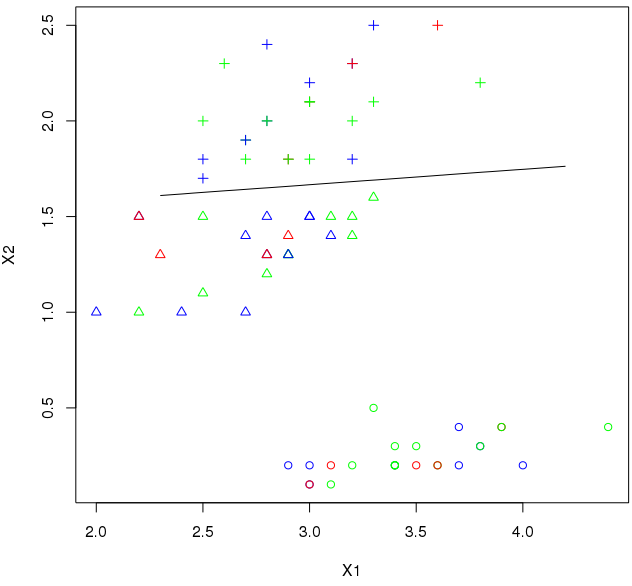
\includegraphics[scale=0.4]{image/q5_1.png}
\end{figure}

Nous obtenons un taux de bonne classification de 0.96 pour une fonction de classification quadratique.

\begin{figure}[!ht]
	\center
	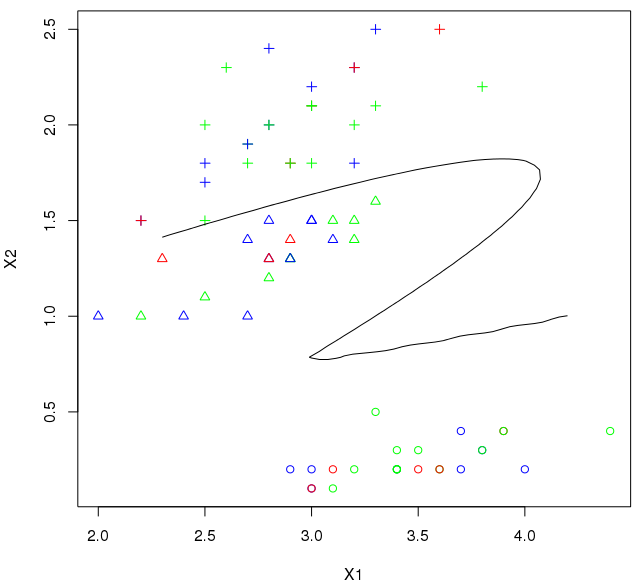
\includegraphics[scale=0.4]{image/q5_2.png}
\end{figure}

On observe que pour des données déjà clairement séparées, la fonction linéaire obtient un taux de classification meilleur que la fonction quadratique. Sur l'image de la fonction quadratique, cette chute du taux de classification est visible car la courbe ne considère pas 2 points (visible à X1=2.5 et X2=1.5)
\newpage
\section*{Question 6}
Nous obtenons un taux de bonne classification de 0.96 pour une fonction de classification linéaire.
\begin{figure}[!ht]
	\center
	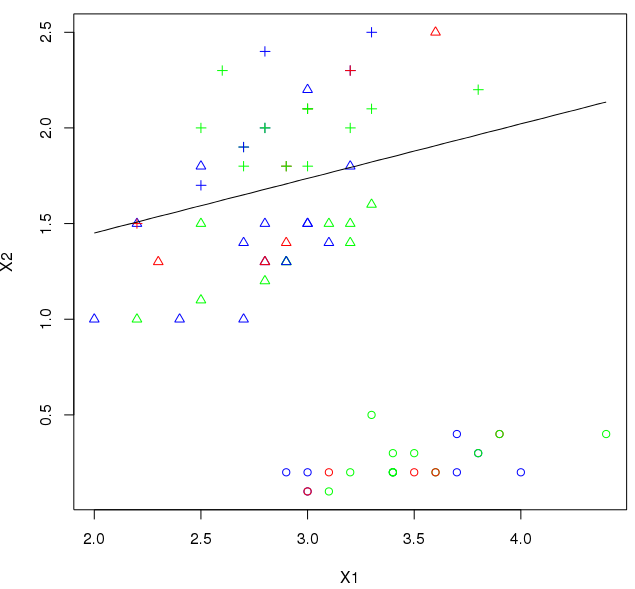
\includegraphics[scale=0.4]{image/q6_1.png}
\end{figure}

Nous obtenons un taux de bonne classification de 0.9466667 pour une fonction de classification quadratique.

\begin{figure}[!ht]
	\center
	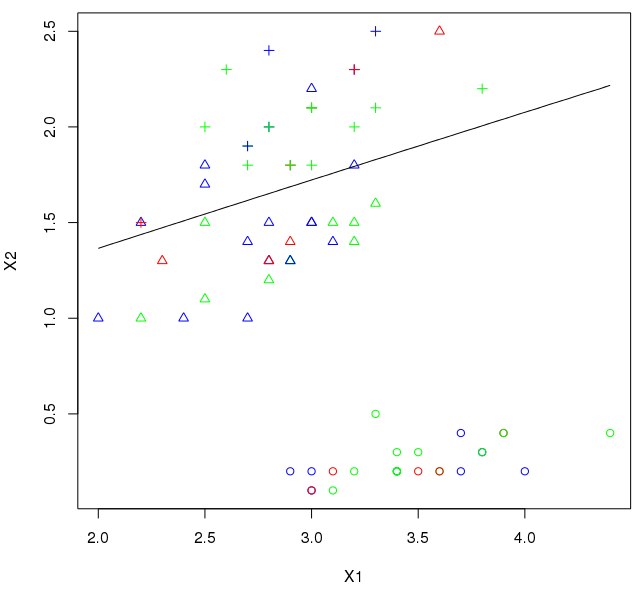
\includegraphics[scale=0.4]{image/q6_2.png}
\end{figure}

On observe qu'en changeant les données test et app, le modèle obtient une base d'apprentissage différente de ce qui est voulue. Que l'on utilise la fonction linéaire ou quadratique n'a donc plus de réelles conséquences sur le taux de classification puisque la classification effectuée par la méthode d'apprentissage n'est pas correcte.

\newpage
\section*{Conclusion}

Dans ce sujet nous avons observé l'importance d'avoir une méthode d'apprentissage pour effectuer une discrimination prcohe d'un taux dit parfait, 1. Nous avons observé les différences entre les fonctions linéaire et quadratique. L'utilisation de la fonction linéaire est préférable lorsque les données sont déjà triées, tandis que la fonction quadratique est plus efficace et permet une meilleur discrimination des données quand celles-ci ne sont pas ordonnées.

En combinant ces techniques nous sommes maintenant capable de discriminer correctement plusieurs zones dans un ensemble de données.

\end{document}
